\chapter{语法}
\section{Node}
\subsection{节点基础}

Node 是一个带有文字的简单图形(矩形,圆形,点)。Node 不属于 path,通常在 path 已经绘制好后,或绘制之前产生。

Node 的最简单用法是在一些坐标点周围添加文字。与此同时,Node也能添加图案以及复杂的颜色效果,甚至一些Node取消了文字。

添加 Node 并没有专用的 \LaTeX 语法,通常用在 path 中用 node 指明。

\begin{figure}[H]
    \centering
    \begin{minipage}{0.35\linewidth}
        \centering
        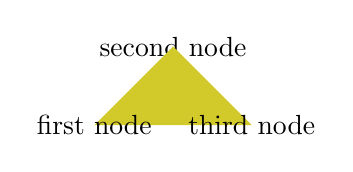
\begin{tikzpicture}[scale = 1]
            \fill [fill=yellow!80!black]
                    (0,0) node  {first node}
                --  (1,1) node[behind path]  {second node}
                --  (2,0) node  {third node};
        \end{tikzpicture}
    \end{minipage}
    \begin{minipage}{0.55\linewidth}
        \begin{lstlisting}[style = latex-side]
    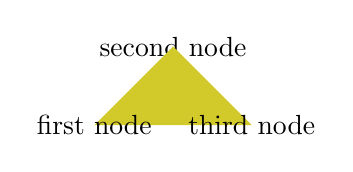
\begin{tikzpicture}[scale = 1]
        \fill [fill=yellow!80!black]
                (0,0) node  {first node}
            --  (1,1) node[behind path]  {second node}
            --  (2,0) node  {third node};
    \end{tikzpicture}
        \end{lstlisting}
    \end{minipage}
    \caption{Node 基本用法}
    \label{Node 基本用法}
\end{figure}

\subsubsection{Node 命令的语法}

\noindent 在 path 中添加 node 的完整语法如下:

\begin{lstlisting}[style = latex]
    \path … node <foreach statements> [<options>] (<name>) at(<coordinate>) :(animation attribute)={<options>} {<node contents>} …;
\end{lstlisting}

\noindent 另一种轻量化的写法

\begin{lstlisting}[style = latex]
    \node [<options>]  (<name>) at(<coordinate>) :(animation);
\end{lstlisting}


\noindent\textbf{主要用法} 
\begin{lstlisting}[style = latex]
    ... node [options] {text} ...;
\end{lstlisting}

\noindent 在 {text} 中添加 node 要显示的文字,[options] 指定样式,下面整理常用 [options]。

\begin{itemize}
    \item 文字与颜色 \\
    除了在 {text} 中指明颜色,在 [options] 也可以使用 [node contents=<text>] 指定文字,且在 [options] 中说明的颜色默认为文字颜色。
    \begin{figure}[H]
        \centering
        \begin{minipage}{0.35\linewidth}
            \centering
            \begin{tikzpicture}[scale = 1]
                \path   (0,0)   node    [blue]  {A}
                        (1,0)   node    [red]   {B}
                        (2,0)   node    [green,node contents=C]
                        (3,0)   node    [node contents=D];
            \end{tikzpicture}
        \end{minipage}
        \begin{minipage}{0.55\linewidth}
            \begin{lstlisting}[style = latex-side]
    \begin{tikzpicture}[scale = 1]
        \path   (0,0)   node    [blue]  {A}
                (1,0)   node    [red]   {B}
                (2,0)   node    [green,node contents=C]
                (3,0)   node    [node contents=D];
    \end{tikzpicture}
            \end{lstlisting}
        \end{minipage}
        \caption{Node 的文字与颜色}
    \end{figure}

    \item 指定位置 \\
    平面位置:[at=<coordinate>]:指定 node 的位置,当 node 在 path 中时,无效。 \\
    图层位置:[behind path]:指定 node 的图层位置,效果见图\ref{Node 基本用法}。默认样式为 [in front of path]

    \item 节点名 \\
    节点名用于后续绘图指定节点,TikZ 允许至多两个节点名。 \\
    节点名:[name=<name>]:节点的名称 \\
    节点别名:[alias=<alias>]:节点别名

    \item 节点形状 \\
    默认节点仅有文字,不具有形状,需要使用 [draw/fill] 命令指定对应形状。\\
    边框:[draw]:显示节点边线;\\
    底色:[fill=<color>]:显示节点底色 \\
    边框形状:[shape = rectangle,circle,ellipse]:shape 可以省略,默认为矩形 rectangle ,更多形状可查阅官方资料。\\
    边框圆角:[rounded corners] \\
    边线数量:[double] \\

    \begin{figure}[H]
        \centering
        \begin{minipage}{0.35\linewidth}
            \centering
            \begin{tikzpicture}[scale = 1]
                \fill[fill=yellow!60!black]
                        (0,0) node [draw, rounded corners] {first node}
                    --  (1,1) node [draw, double, ellipse, behind path] {second node}
                    --  (0,2) node [circle,fill=red!20] {third node};
            \end{tikzpicture}
        \end{minipage}
        \begin{minipage}{0.55\linewidth}
            \begin{lstlisting}[style = latex-side]
    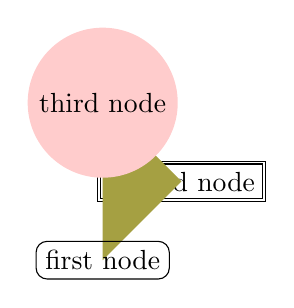
\begin{tikzpicture}[scale = 1]
        \fill[fill=yellow!60!black]
                (0,0) node [draw, rounded corners] {first node}
            --  (1,1) node [draw, double, behind path] {second node}
            --  (0,2) node [circle,fill=red!20] {third node};
    \end{tikzpicture}
            \end{lstlisting}
        \end{minipage}
        \caption{Node 形状}
    \end{figure}

    \item 节点全局样式 \\
    可以通过在 tikzpicture 环境开始处添加说明,给予全局节点样式。\\
    全部样式:[every node/.style = \{\}]\\
    \begin{figure}[H]
        \centering
        \begin{minipage}{0.35\linewidth}
            \centering
            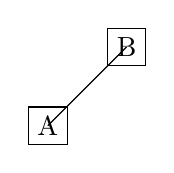
\begin{tikzpicture}[every node/.style={draw}]
                \draw (0,0) node {A} -- (1,1) node {B};
            \end{tikzpicture}
        \end{minipage}
        \begin{minipage}{0.55\linewidth}
            \begin{lstlisting}[style = latex-side]
    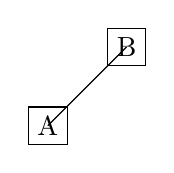
\begin{tikzpicture}[every node/.style={draw}]
        \draw (0,0) node {A} -- (1,1) node {B};
    \end{tikzpicture}
            \end{lstlisting}
        \end{minipage}
        \caption{Node 全部样式}
    \end{figure}
    指定样式:[every <shape> node/.style = \{\}]\\
    \begin{figure}[H]
        \centering
        \begin{minipage}{0.35\linewidth}
            \centering
            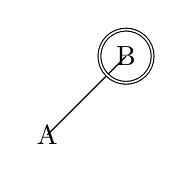
\begin{tikzpicture}[every circle node/.style={draw,double}]
                \draw   (0,0)   node    {A} 
                    --  (1,1)   [circle] node {B};
            \end{tikzpicture}
        \end{minipage}
        \begin{minipage}{0.55\linewidth}
            \begin{lstlisting}[style = latex-side]
    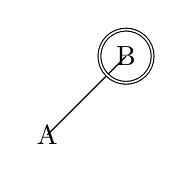
\begin{tikzpicture}[every circle node/.style={draw,double}]
        \draw   (0,0)   node    {A} 
            --  (1,1)   [circle] node {B};
    \end{tikzpicture}
            \end{lstlisting}
        \end{minipage}
        \caption{Node 指定样式}
    \end{figure}
    文字前后缀:[execute at begin/end node = \{text\}] \\
    \begin{figure}[H]
        \centering
        \begin{minipage}{0.35\linewidth}
            \centering
            \begin{tikzpicture}[execute at begin node = {第}, execute at end node = {题}]
                \node [execute at end node = {:}] {一};
            \end{tikzpicture}
        \end{minipage}
        \begin{minipage}{0.55\linewidth}
            \begin{lstlisting}[style = latex-side]
    \begin{tikzpicture}[execute at begin node = {第}, execute at end node = {题}]
        \node [execute at end node = {:}] {一};
    \end{tikzpicture}
            \end{lstlisting}
        \end{minipage}
        \caption{}
    \end{figure}

    \item 其他样式 \\
    填充:[fill = <color>]:填充背景色 \\
    缩放:[scale = <dimension>]:节点缩放 \\
    边框粗细:[linewidth = <dimension>]:边框粗细 \\

\end{itemize}

\noindent\textbf{其他用法} 
\begin{itemize}
    \item 节点动画 \\
    \noindent 通过 :<animation attribute>={<options>},可以设定动画\footnote{部分图形驱动并不支持动画,比如我的也不支持},下面只做简单举例 \\
    \begin{figure}[H]
        \centering
        \begin{minipage}{0.35\linewidth}
            \centering
            \begin{tikzpicture}[scale = 1]
                \node   :fill opacity={0s="1",2s="0",begin on=click}
                        :rotate = {0s="0",2s="90",begin on=click}
                        [fill = blue!20, draw = blue, ultra thick, circle]
                        {click me};
            \end{tikzpicture}
        \end{minipage}
        \begin{minipage}{0.55\linewidth}
            \begin{lstlisting}[style = latex-side]
        \begin{tikzpicture}[scale = 1]
            \node   :fill opacity={0s="1",2s="0",begin on=click}
                    :rotate = {0s="0",2s="90",begin on=click}
                    [fill = blue!20, draw = blue, ultra thick, circle]
                    {click me};
        \end{tikzpicture}
            \end{lstlisting}
        \end{minipage}
        \caption{Node 动画}
    \end{figure}

    \item foreach \\
    foreach 语句仅允许紧跟在 node 之后出现。\\
    语法形式:foreach \textbackslash x in \{\}\\
    在集合{}中可以使用 ... 表示省略类似的内容。\\


    \begin{figure}[H]
        \centering
        \begin{minipage}{0.35\linewidth}
            \centering
            \begin{tikzpicture}[scale = 1]
                \draw (0,0) node foreach \x in {1,2,3} at (\x,0) {\x};
            \end{tikzpicture}
        \end{minipage}
        \begin{minipage}{0.55\linewidth}
            \begin{lstlisting}[style = latex-side]
    % 以下两句效果相同
    \draw (0,0) node foreach \x in {1,2,3} at (\x,0) {\x};
    \tikz \draw (0,0) node at (1,0) {1} node at (2,0) {2} node at (3,0) {3};
            \end{lstlisting}
        \end{minipage}
        \caption{Node 一次迭代}
    \end{figure}

    \begin{figure}[H]
        \centering
        \begin{minipage}{0.35\linewidth}
            \centering
            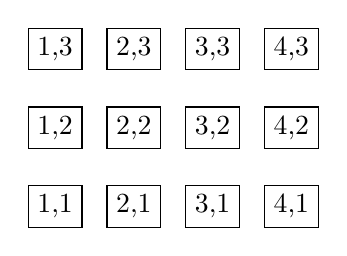
\begin{tikzpicture}[scale = 1]
                \node foreach \x in {1,...,4} foreach \y in {1,2,3} [draw] at (\x,\y) {\x,\y};
            \end{tikzpicture}
        \end{minipage}
        \begin{minipage}{0.55\linewidth}
            \begin{lstlisting}[style = latex-side]
    \node foreach \x in {1,...,4} foreach \y in {1,2,3} [draw] at (\x,\y) {\x,\y};
            \end{lstlisting}
        \end{minipage}
        \caption{Node 两次迭代}
    \end{figure}

    \item scope \\
    scope 用于限定范围,类似高级语言中的命名空间。\\
    和 \LaTeX 中的环境十分相似,scope需要 \textbackslash begin 和 \textbackslash end 来限定范围。\\
    在 \textbackslash begin\{scope\}[name prefix = <text>] 限定范围名。\\
    使用时 "name"+"node name" 即可。\\
    类似的,也可以使用 suffix。 \\
    \begin{figure}[H]
        \centering
        \begin{minipage}{0.35\linewidth}
            \centering
            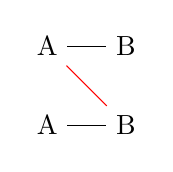
\begin{tikzpicture}[scale = 1]
                \begin{scope}[name prefix = top-]
                    \node (A) at (0,1) {A};
                    \node (B) at (1,1) {B};
                    \draw (A) -- (B);
                \end{scope}
                \begin{scope}[name prefix = buttom-]
                    \node (A) at (0,0) {A};
                    \node (B) at (1,0) {B};
                    \draw (A) -- (B);
                \end{scope}
                \draw [red] (top-A) -- (buttom-B);
            \end{tikzpicture}
        \end{minipage}
        \begin{minipage}{0.55\linewidth}
            \begin{lstlisting}[style = latex-side]
    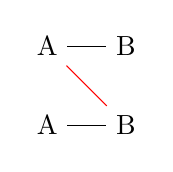
\begin{tikzpicture}[scale = 1]
        \begin{scope}[name prefix = top-]
            \node (A) at (0,1) {A};
            \node (B) at (1,1) {B};
            \draw (A) -- (B);
        \end{scope}
        \begin{scope}[name prefix = buttom-]
            \node (A) at (0,0) {A};
            \node (B) at (1,0) {B};
            \draw (A) -- (B);
        \end{scope}
        \draw [red] (top-A) -- (buttom-B);
    \end{tikzpicture}
            \end{lstlisting}
        \end{minipage}
        \caption{Node:sep}
    \end{figure}
\end{itemize}

\subsubsection{盒模型}

盒模型\footnote{盒模型概念来自css,与这里极其类使,但 TikZ 官方并没有指定这一系列样式的名称},这里指 Node 周围边距,底色等样式的控制。由于比一般的样式控制命令更多,而且重要,单独开一节做笔记。

\begin{itemize}
    \item 边距 sep \hfill(默认: 0.3333em) \\
    总内边距:[inner sep = <dimension>]:边框与内部文字的边距
    \begin{figure}[H]
        \centering
        \begin{minipage}{0.35\linewidth}
            \centering
            \begin{tikzpicture}[scale = 1]
                \draw   (0,0) node [inner sep = 0pt,draw] {0pt}
                        (0,2em) node [inner sep = 5pt,draw] {5pt}
                        (0,4em) node [draw]  {默认};
            \end{tikzpicture}
        \end{minipage}
        \begin{minipage}{0.55\linewidth}
            \begin{lstlisting}[style = latex-side]
    \begin{tikzpicture}[scale = 1]
        \draw   (0,0) node [inner sep = 0pt,draw] {0pt}
                (0,2em) node [inner sep = 5pt,draw] {5pt}
                (0,4em) node [draw]  {默认};
    \end{tikzpicture}
            \end{lstlisting}
        \end{minipage}
        \caption{Node:inner sep}
    \end{figure}

    左右/上下边距:[inner xsep/ysep = <dimension>]\\
    外边距:[outer sep = <dimension>],外边距可能出现一些不准确的问题,可以在环境中加入 [outer sep = auto] 解决,与 inner sep 类使的,也可以指明 x/y 方向外边距。

    \item 最小高度/宽度 \\
    最小高度/宽度用于限制节点与边线的最小距离 \\
    最小距离:[minimum size]:最小高度与宽度 \\
    最小高度:[minimum height], 最小宽度:[minimum width]
    \begin{figure}[H]
        \centering
        \begin{minipage}{0.35\linewidth}
            \centering
            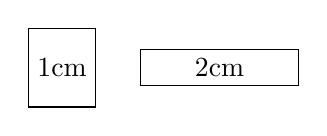
\begin{tikzpicture}[scale = 1]
                \draw   (0,0)   node    [minimum height = 1cm,draw] {1cm}
                        (2,0)   node    [minimum width = 2cm,draw] {2cm};
            \end{tikzpicture}
        \end{minipage}
        \begin{minipage}{0.55\linewidth}
            \begin{lstlisting}[style = latex-side]
    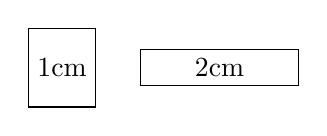
\begin{tikzpicture}[scale = 1]
        \draw   (0,0)   node    [minimum height = 1cm,draw] {1cm}
                (2,0)   node    [minimum width = 2cm,draw] {2cm};
    \end{tikzpicture}
            \end{lstlisting}
        \end{minipage}
        \caption{Node:最小高度/宽度}
    \end{figure}
\end{itemize}

\subsubsection{边框形状}
这里主要备注边框形状相关的内容。
\begin{itemize}
    \item 横纵比 \\
    横纵比:[shape aspect=<aspect ratio>]:外边框形状进行压缩。
    \begin{figure}[H]
        \centering
        \begin{minipage}{0.35\linewidth}
            \centering
            \begin{tikzpicture}[scale = 1]
                \draw   (0,0)   node    [shape aspect=1,diamond,draw] {aspect 1};
                \draw   (0,-2)  node    [shape aspect=2,diamond,draw] {aspect 2};
            \end{tikzpicture}
        \end{minipage}
        \begin{minipage}{0.55\linewidth}
            \begin{lstlisting}[style = latex-side]
    \begin{tikzpicture}[scale = 1]
        \draw   (0,0)   node    [shape aspect=1,diamond,draw] {aspect 1};
        \draw   (0,-2)  node    [shape aspect=2,diamond,draw] {aspect 2};
    \end{tikzpicture}
            \end{lstlisting}
        \end{minipage}
        \caption{Node:aspect}
    \end{figure}

    \item 边框距 \hfill (默认: 1pt)\\
    TikZ 的边框距有两种计算方式,可以使用 [shape border uses incircle = <boolean>] 启动第二种边距计算,效果见下图:
    \begin{figure}[H]
        \centering
        \begin{minipage}{0.35\linewidth}
            \centering
            \begin{tikzpicture}[every node/.style = {isosceles triangle,draw}]
                \node at (0,0) {abc};
                \node [shape border uses incircle] at (2,0) {abc};
                \node [circle,minimum size = 2em] at (0,0) {}; 
                \node [circle,minimum size = 2em] at (2,0) {}; 
            \end{tikzpicture}
        \end{minipage}
        \begin{minipage}{0.55\linewidth}
            \begin{lstlisting}[style = latex-side]
        
            \end{lstlisting}
        \end{minipage}
        \caption{Node:边距}
    \end{figure}

    \item 旋转 \\
    文字旋转:[rotate = <angle>]:文字和边框都将出现旋转。\\
    边框旋转:[rotate = <angle>]:仅边框旋转。 \\
    \begin{figure}[H]
        \centering
        \begin{minipage}{0.35\linewidth}
            \centering
            \begin{tikzpicture}[every node/.style={shape=trapezium, draw, shape border uses incircle}]
                \node at (0,0) (A) {A};
                \node [shape border rotate=30] at (1.5,0) {B};
                \node [rotate=30] at (3,0) {C};
            \end{tikzpicture}
        \end{minipage}
        \begin{minipage}{0.55\linewidth}
            \begin{lstlisting}[style = latex-side]
    \begin{tikzpicture}[every node/.style={shape=trapezium, draw, shape border usincircle}]
        \node at (0,0) (A) {A};
        \node [shape border rotate=30] at (1.5,0) {B};
        \node [rotate=30] at (3,0) {C};
    \end{tikzpicture}
            \end{lstlisting}
        \end{minipage}
        \caption{Node:旋转}
    \end{figure}

    \item 边框粗细 \\
    粗细:[linewidth = <dimension>]
    \begin{figure}[H]
        \centering
        \begin{minipage}{0.35\linewidth}
            \centering
            
\begin{tikzpicture}[scale = 1]
                \node [line width=2,draw] at (0,0) {A};
            \end{tikzpicture}
        \end{minipage}
        \begin{minipage}{0.55\linewidth}
            \begin{lstlisting}[style = latex-side]
    
\begin{tikzpicture}[scale = 1]
        \node [line width=2,draw] at (0,0) {A};
    \end{tikzpicture}
            \end{lstlisting}
        \end{minipage}
        \caption{Node:边框粗细}
    \end{figure}
\end{itemize}

\subsection{节点样式}
\subsubsection{分割节点}
在 node 文字{}中使用 \verb|\|nodepart[<options>]\{<part name>\} 可以对节点进行切割;注意此时的 shape 形状后需加上 split,否则无效。同时需要声明 \verb|\|use tikzlibrary {shapes.multipart}

\begin{figure}[H]
    \centering
    \begin{minipage}{0.35\linewidth}
        \centering
        \begin{tikzpicture}[scale = 1]
            \node [circle split,draw,double] {$q_1$ \nodepart{lower} $00$};
        \end{tikzpicture}
    \end{minipage}
    \begin{minipage}{0.55\linewidth}
        \begin{lstlisting}[style = latex-side]
    \begin{tikzpicture}[scale = 1]
        \node [circle split,draw,double] {$q_1$ \nodepart{lower} $00$};
    \end{tikzpicture}
        \end{lstlisting}
    \end{minipage}
    \caption{Node:分割节点}
\end{figure}

对于批量修改节点样式,可以使用类似 every lower node part/.style = color 的方法。

\begin{figure}[H]
    \centering
    \begin{minipage}{0.35\linewidth}
        \centering
        \begin{tikzpicture}[every lower node part/.style = red]
            \node [circle split,draw] {$q_1$ \nodepart{lower} $00$};
        \end{tikzpicture}
    \end{minipage}
    \begin{minipage}{0.55\linewidth}
        \begin{lstlisting}[style = latex-side]
    \begin{tikzpicture}[every lower node part/.style = red]
        \node [circle split,draw] {$q_1$ \nodepart{lower} $00$};
    \end{tikzpicture}
        \end{lstlisting}
    \end{minipage}
    \caption{Node:分割节点样式}
\end{figure}

\subsubsection{节点文字}

文字本身包含颜色,字体,大小等样式,具体控制如下:
\begin{itemize}
    \item 颜色 \\
    文字颜色:[color = <color>],这里的color可以省略,注意在节点中的颜色属性只影响节点文字,这与 \verb|\|draw 不同

    \begin{figure}[H]
        \centering
        \begin{minipage}{0.35\linewidth}
            \centering
            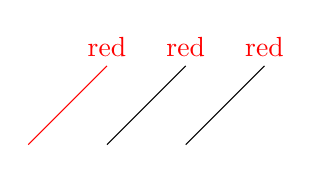
\begin{tikzpicture}[scale = 1]
                \draw[red]          (0,0) -- +(1,1) node[above] {red};
                \draw[text = red]   (1,0) -- +(1,1) node[above] {red};
                \draw               (2,0) -- +(1,1) node[above,red] {red};
            \end{tikzpicture}
        \end{minipage}
        \begin{minipage}{0.55\linewidth}
            \begin{lstlisting}[style = latex-side]
    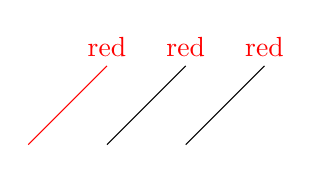
\begin{tikzpicture}[scale = 1]
        \draw[red]          (0,0) -- +(1,1) node[above] {red};
        \draw[text = red]   (1,0) -- +(1,1) node[above] {red};
        \draw               (2,0) -- +(1,1) node[above,red] {red};
    \end{tikzpicture}
            \end{lstlisting}
        \end{minipage}
        \caption{Node:文字颜色}
    \end{figure}

    \item 不透明度 \\
    不透明度:[opacity = <value>],注意这里是不透明度,1表示完全不透明。

    \begin{figure}[H]
        \centering
        \begin{minipage}{0.35\linewidth}
            \centering
            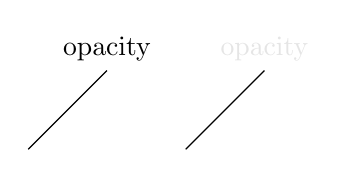
\begin{tikzpicture}[scale = 1]
                \draw[opacity = 1]          (0,0) -- +(1,1) node[above] {opacity};
                \draw               (2,0) -- +(1,1) node[above,opacity = 0.1] {opacity};
            \end{tikzpicture}
        \end{minipage}
        \begin{minipage}{0.55\linewidth}
            \begin{lstlisting}[style = latex-side]
    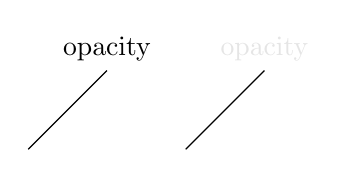
\begin{tikzpicture}[scale = 1]
        \draw[opacity = 1]          (0,0) -- +(1,1) node[above] {opacity};
        \draw               (2,0) -- +(1,1) node[above,opacity = 0.1] {opacity};
    \end{tikzpicture}
            \end{lstlisting}
        \end{minipage}
        \caption{Node:文字透明度}
    \end{figure}

    \item 文字字体 \\
    文字字体:[node font = <font commands>],这里的 node 可以省略。注意这里的 font 既可以指字体族,也可以控制字体大小。

    \begin{figure}[H]
        \centering
        \begin{minipage}{0.35\linewidth}
            \centering
            \begin{tikzpicture}[every text node part/.style={font=\itshape},every lower node part/.style={font=\footnotesize}]
                \draw[node font=\itshape] (1,0) -- +(1,1) node[above] {italic};
                \draw[node font=\tiny] (2,0) -- +(1,1) node[above] {tiny};
                \node [circle split,draw] at (4,0) {state \nodepart{lower} output};
            \end{tikzpicture}
        \end{minipage}
        \begin{minipage}{0.55\linewidth}
            \begin{lstlisting}[style = latex-side]
    \begin{tikzpicture}[every text node part/.style={font=\itshape},every lower node part/.style={font=\footnotesize}]
        \draw[node font=\itshape] (1,0) -- +(1,1) node[above] {italic};
        \draw[node font=\tiny] (2,0) -- +(1,1) node[above] {tiny};
        \node [circle split,draw] at (4,0) {state \nodepart{lower} output};
    \end{tikzpicture}
            \end{lstlisting}
        \end{minipage}
        \caption{Node:文字字体}
    \end{figure}

    \item 文字高度与深度 \\
    文字高度:[text height = <dimension>] \\
    文字深度:[text depth = <dimension>] \\
    这两个属性并不常用,一般情况下尽量用 inner sep 代替。
\end{itemize}

\subsubsection{节点文本}

文本格式包括文本框的长宽,对齐方式等。

\begin{itemize}
    \item 节点文本框\\
    与正文中的文本类似,节点中的文本也可以实现公式,换行,表格等功能。

    \begin{figure}[H]
        \centering
        \begin{minipage}{0.35\linewidth}
            \centering
            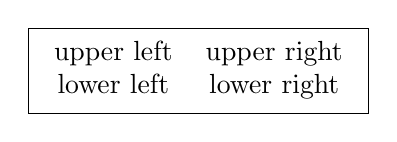
\begin{tikzpicture}[scale = 1]
                \node [draw] {
                    \begin{tabular}{cc}
                        upper left & upper right\\
                        lower left & lower right
                    \end{tabular}
                };
            \end{tikzpicture}
        \end{minipage}
        \begin{minipage}{0.55\linewidth}
            \begin{lstlisting}[style = latex-side]
    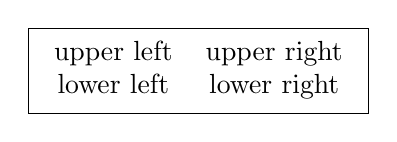
\begin{tikzpicture}[scale = 1]
        \node [draw] {
            \begin{tabular}{cc}
                upper left & upper right\\
                lower left & lower right
            \end{tabular}
        };
    \end{tikzpicture}
            \end{lstlisting}
        \end{minipage}
        \caption{Node:节点文本框}
    \end{figure}

    \item 文本对齐\\
    对齐:[align = <alignment option>],设置对其方式。

    \begin{figure}[H]
        \centering
        \begin{minipage}{0.35\linewidth}
            \centering
            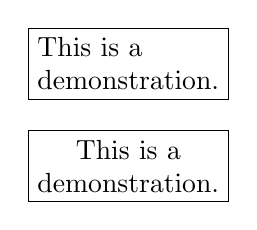
\begin{tikzpicture}[scale = 1]
                \node[draw,align=left]at (0,0) {This is a\\demonstration.};
                \node[draw,align=center] at (0,-1.3) {This is a\\demonstration.};
            \end{tikzpicture}
        \end{minipage}
        \begin{minipage}{0.55\linewidth}
            \begin{lstlisting}[style = latex-side]
    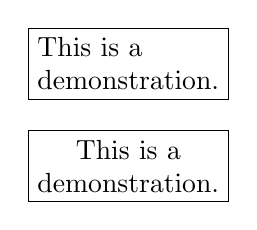
\begin{tikzpicture}[scale = 1]
        \node[draw,align=left]at (0,0) {This is a\\demonstration.};
        \node[draw,align=center] at (0,-1.3) {This is a\\demonstration.};
    \end{tikzpicture}
            \end{lstlisting}
        \end{minipage}
        \caption{Node:文本对齐}
    \end{figure}

    \noindent 文本对齐会自动分割长单词,可以使用 align = flush <alignment option> 来取消长单词。
    \begin{figure}[H]
        \centering
        \begin{minipage}{0.35\linewidth}
            \centering
            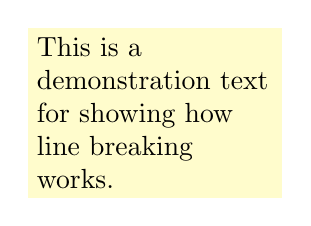
\begin{tikzpicture}[scale = 1]
                \node[fill=yellow!20,text width=3cm,align=flush left] {This is a demonstration text for showing how line breaking works.};
            \end{tikzpicture}
        \end{minipage}
        \begin{minipage}{0.55\linewidth}
            \begin{lstlisting}[style = latex-side]
    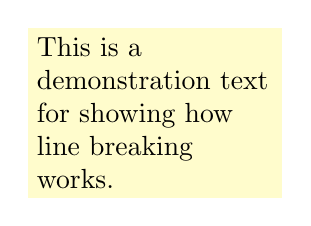
\begin{tikzpicture}[scale = 1]
        \node[fill=yellow!20,text width=3cm,align=flush left] {This is a demonstration text for showing how line breaking works.};
    \end{tikzpicture}
            \end{lstlisting}
        \end{minipage}
        \caption{Node:分割长单词}
    \end{figure}

    alignment option 具体参数见属性百科:

    \item 文本宽度 \\
    文本宽:[text width = <dimension>]:限定最大文本宽

    \begin{figure}[H]
        \centering
        \begin{minipage}{0.35\linewidth}
            \centering
            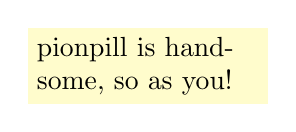
\begin{tikzpicture}[scale = 1]
                \draw (0,0) node [text width=8em, fill = yellow!20] {pionpill is handsome, so as you!};
            \end{tikzpicture}
        \end{minipage}
        \begin{minipage}{0.55\linewidth}
            \begin{lstlisting}[style = latex-side]
    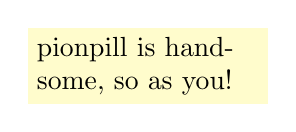
\begin{tikzpicture}[scale = 1]
        \draw (0,0) node [text width=8em, fill = yellow!20] {pionpill is handsome, so as you!};
    \end{tikzpicture}
            \end{lstlisting}
        \end{minipage}
        \caption{Node:文本宽度}
    \end{figure}
\end{itemize}

\subsection{节点布局}
\subsubsection{定位}

节点的未知往往由与之相关的坐标决定,默认以坐标为中心生成节点,同时也可在坐标周围生成节点。
